% BEGIN EDITOR ASSETS (generated by code/sync_paper_assets.py)
\begin{filecontents*}{neurips_2025.sty}
% partial rewrite of the LaTeX2e package for submissions to the
% Conference on Neural Information Processing Systems (NeurIPS):
%
% - uses more LaTeX conventions
% - line numbers at submission time replaced with aligned numbers from
%   lineno package
% - \nipsfinalcopy replaced with [final] package option
% - automatically loads times package for authors
% - loads natbib automatically; this can be suppressed with the
%   [nonatbib] package option
% - adds foot line to first page identifying the conference
% - adds preprint option for submission to e.g. arXiv
% - conference acronym modified
% - update foot line to display the track name
%
% Roman Garnett (garnett@wustl.edu) and the many authors of
% nips15submit_e.sty, including MK and drstrip@sandia
%
% last revision: April 2025

\NeedsTeXFormat{LaTeX2e}
\ProvidesPackage{neurips_2025}[2025/05/01 NeurIPS 2025 submission/camera-ready style file]

% declare final option, which creates camera-ready copy
\newif\if@neuripsfinal\@neuripsfinalfalse
\DeclareOption{final}{
  \@neuripsfinaltrue
  \@anonymousfalse
}

% declare nonatbib option, which does not load natbib in case of
% package clash (users can pass options to natbib via
% \PassOptionsToPackage)
\newif\if@natbib\@natbibtrue
\DeclareOption{nonatbib}{
  \@natbibfalse
}

% declare preprint option, which creates a preprint version ready for
% upload to, e.g., arXiv
\newif\if@preprint\@preprintfalse
\DeclareOption{preprint}{
  \@preprinttrue
  \@anonymousfalse
}

% determine the track of the paper in camera-ready mode
\newif\if@main\@maintrue
\DeclareOption{main}{
  \@maintrue
  \newcommand{\@trackname}{\@neuripsordinal\ Conference on Neural Information Processing Systems (NeurIPS \@neuripsyear).}
}
\newif\if@position\@positionfalse
\DeclareOption{position}{
  \@positiontrue
  \newcommand{\@trackname}{\@neuripsordinal\ Conference on Neural Information Processing Systems (NeurIPS \@neuripsyear) Position Paper Track.}
}
\newif\if@dandb\@dandbfalse
\DeclareOption{dandb}{
  \@dandbtrue
  \@anonymousfalse
  \newcommand{\@trackname}{\@neuripsordinal\ Conference on Neural Information Processing Systems (NeurIPS \@neuripsyear) Track on Datasets and Benchmarks.}
}
\newif\if@creativeai\@creativeaifalse
\DeclareOption{creativeai}{
  \@creativeaitrue
  \@anonymousfalse
  \newcommand{\@trackname}{\@neuripsordinal\ Conference on Neural Information Processing Systems (NeurIPS \@neuripsyear) Creative AI Track.}
}

% For anonymous or non-anonymous
\newif\if@anonymous\@anonymoustrue

% For workshop papers
\newcommand{\@workshoptitle}{}
\newcommand{\workshoptitle}[1]{\renewcommand{\@workshoptitle}{#1}}

\newif\if@workshop\@workshopfalse
\DeclareOption{sglblindworkshop}{
  \@workshoptrue
  \@anonymousfalse
  \newcommand{\@trackname}{\@neuripsordinal\ Conference on Neural Information Processing Systems (NeurIPS \@neuripsyear) Workshop: \@workshoptitle.}
}
\DeclareOption{dblblindworkshop}{
  \@workshoptrue
  \newcommand{\@trackname}{\@neuripsordinal\ Conference on Neural Information Processing Systems (NeurIPS \@neuripsyear) Workshop: \@workshoptitle.}
}

\ProcessOptions\relax

% fonts
\renewcommand{\rmdefault}{ptm}
\renewcommand{\sfdefault}{phv}

% change this every year for notice string at bottom
\newcommand{\@neuripsordinal}{39th}
\newcommand{\@neuripsyear}{2025}
\newcommand{\@neuripslocation}{San Diego}

% acknowledgments
\usepackage{environ}
\newcommand{\acksection}{\section*{Acknowledgments and Disclosure of Funding}}
\NewEnviron{ack}{%
  \acksection
  \BODY
}


% load natbib unless told otherwise
\if@natbib
  \RequirePackage{natbib}
\fi

% set page geometry
\usepackage[verbose=true,letterpaper]{geometry}
\AtBeginDocument{
  \newgeometry{
    textheight=9in,
    textwidth=5.5in,
    top=1in,
    headheight=12pt,
    headsep=25pt,
    footskip=30pt
  }
  \@ifpackageloaded{fullpage}
    {\PackageWarning{neurips_2025}{fullpage package not allowed! Overwriting formatting.}}
    {}
}

\widowpenalty=10000
\clubpenalty=10000
\flushbottom
\sloppy


% font sizes with reduced leading
\renewcommand{\normalsize}{%
  \@setfontsize\normalsize\@xpt\@xipt
  \abovedisplayskip      7\p@ \@plus 2\p@ \@minus 5\p@
  \abovedisplayshortskip \z@ \@plus 3\p@
  \belowdisplayskip      \abovedisplayskip
  \belowdisplayshortskip 4\p@ \@plus 3\p@ \@minus 3\p@
}
\normalsize
\renewcommand{\small}{%
  \@setfontsize\small\@ixpt\@xpt
  \abovedisplayskip      6\p@ \@plus 1.5\p@ \@minus 4\p@
  \abovedisplayshortskip \z@  \@plus 2\p@
  \belowdisplayskip      \abovedisplayskip
  \belowdisplayshortskip 3\p@ \@plus 2\p@   \@minus 2\p@
}
\renewcommand{\footnotesize}{\@setfontsize\footnotesize\@ixpt\@xpt}
\renewcommand{\scriptsize}{\@setfontsize\scriptsize\@viipt\@viiipt}
\renewcommand{\tiny}{\@setfontsize\tiny\@vipt\@viipt}
\renewcommand{\large}{\@setfontsize\large\@xiipt{14}}
\renewcommand{\Large}{\@setfontsize\Large\@xivpt{16}}
\renewcommand{\LARGE}{\@setfontsize\LARGE\@xviipt{20}}
\renewcommand{\huge}{\@setfontsize\huge\@xxpt{23}}
\renewcommand{\Huge}{\@setfontsize\Huge\@xxvpt{28}}

% sections with less space
\providecommand{\section}{}
\renewcommand{\section}{%
  \@startsection{section}{1}{\z@}%
                {-2.0ex \@plus -0.5ex \@minus -0.2ex}%
                { 1.5ex \@plus  0.3ex \@minus  0.2ex}%
                {\large\bf\raggedright}%
}
\providecommand{\subsection}{}
\renewcommand{\subsection}{%
  \@startsection{subsection}{2}{\z@}%
                {-1.8ex \@plus -0.5ex \@minus -0.2ex}%
                { 0.8ex \@plus  0.2ex}%
                {\normalsize\bf\raggedright}%
}
\providecommand{\subsubsection}{}
\renewcommand{\subsubsection}{%
  \@startsection{subsubsection}{3}{\z@}%
                {-1.5ex \@plus -0.5ex \@minus -0.2ex}%
                { 0.5ex \@plus  0.2ex}%
                {\normalsize\bf\raggedright}%
}
\providecommand{\paragraph}{}
\renewcommand{\paragraph}{%
  \@startsection{paragraph}{4}{\z@}%
                {1.5ex \@plus 0.5ex \@minus 0.2ex}%
                {-1em}%
                {\normalsize\bf}%
}
\providecommand{\subparagraph}{}
\renewcommand{\subparagraph}{%
  \@startsection{subparagraph}{5}{\z@}%
                {1.5ex \@plus 0.5ex \@minus 0.2ex}%
                {-1em}%
                {\normalsize\bf}%
}
\providecommand{\subsubsubsection}{}
\renewcommand{\subsubsubsection}{%
  \vskip5pt{\noindent\normalsize\rm\raggedright}%
}

% float placement
\renewcommand{\topfraction      }{0.85}
\renewcommand{\bottomfraction   }{0.4}
\renewcommand{\textfraction     }{0.1}
\renewcommand{\floatpagefraction}{0.7}

\newlength{\@neuripsabovecaptionskip}\setlength{\@neuripsabovecaptionskip}{7\p@}
\newlength{\@neuripsbelowcaptionskip}\setlength{\@neuripsbelowcaptionskip}{\z@}

\setlength{\abovecaptionskip}{\@neuripsabovecaptionskip}
\setlength{\belowcaptionskip}{\@neuripsbelowcaptionskip}

% swap above/belowcaptionskip lengths for tables
\renewenvironment{table}
  {\setlength{\abovecaptionskip}{\@neuripsbelowcaptionskip}%
   \setlength{\belowcaptionskip}{\@neuripsabovecaptionskip}%
   \@float{table}}
  {\end@float}

% footnote formatting
\setlength{\footnotesep }{6.65\p@}
\setlength{\skip\footins}{9\p@ \@plus 4\p@ \@minus 2\p@}
\renewcommand{\footnoterule}{\kern-3\p@ \hrule width 12pc \kern 2.6\p@}
\setcounter{footnote}{0}

% paragraph formatting
\setlength{\parindent}{\z@}
\setlength{\parskip  }{5.5\p@}

% list formatting
\setlength{\topsep       }{4\p@ \@plus 1\p@   \@minus 2\p@}
\setlength{\partopsep    }{1\p@ \@plus 0.5\p@ \@minus 0.5\p@}
\setlength{\itemsep      }{2\p@ \@plus 1\p@   \@minus 0.5\p@}
\setlength{\parsep       }{2\p@ \@plus 1\p@   \@minus 0.5\p@}
\setlength{\leftmargin   }{3pc}
\setlength{\leftmargini  }{\leftmargin}
\setlength{\leftmarginii }{2em}
\setlength{\leftmarginiii}{1.5em}
\setlength{\leftmarginiv }{1.0em}
\setlength{\leftmarginv  }{0.5em}
\def\@listi  {\leftmargin\leftmargini}
\def\@listii {\leftmargin\leftmarginii
              \labelwidth\leftmarginii
              \advance\labelwidth-\labelsep
              \topsep  2\p@ \@plus 1\p@    \@minus 0.5\p@
              \parsep  1\p@ \@plus 0.5\p@ \@minus 0.5\p@
              \itemsep \parsep}
\def\@listiii{\leftmargin\leftmarginiii
              \labelwidth\leftmarginiii
              \advance\labelwidth-\labelsep
              \topsep    1\p@ \@plus 0.5\p@ \@minus 0.5\p@
              \parsep    \z@
              \partopsep 0.5\p@ \@plus 0\p@ \@minus 0.5\p@
              \itemsep \topsep}
\def\@listiv {\leftmargin\leftmarginiv
              \labelwidth\leftmarginiv
              \advance\labelwidth-\labelsep}
\def\@listv  {\leftmargin\leftmarginv
              \labelwidth\leftmarginv
              \advance\labelwidth-\labelsep}
\def\@listvi {\leftmargin\leftmarginvi
              \labelwidth\leftmarginvi
              \advance\labelwidth-\labelsep}

% create title
\providecommand{\maketitle}{}
\renewcommand{\maketitle}{%
  \par
  \begingroup
    \renewcommand{\thefootnote}{\fnsymbol{footnote}}
    % for perfect author name centering
    \renewcommand{\@makefnmark}{\hbox to \z@{$^{\@thefnmark}$\hss}}
    % The footnote-mark was overlapping the footnote-text,
    % added the following to fix this problem               (MK)
    \long\def\@makefntext##1{%
      \parindent 1em\noindent
      \hbox to 1.8em{\hss $\m@th ^{\@thefnmark}$}##1
    }
    \thispagestyle{empty}
    \@maketitle
    \@thanks
    \@notice
  \endgroup
  \let\maketitle\relax
  \let\thanks\relax
}

% rules for title box at top of first page
\newcommand{\@toptitlebar}{
  \hrule height 4\p@
  \vskip 0.25in
  \vskip -\parskip%
}
\newcommand{\@bottomtitlebar}{
  \vskip 0.29in
  \vskip -\parskip
  \hrule height 1\p@
  \vskip 0.09in%
}

% create title (includes both anonymized and non-anonymized versions)
\providecommand{\@maketitle}{}
\renewcommand{\@maketitle}{%
  \vbox{%
    \hsize\textwidth
    \linewidth\hsize
    \vskip 0.1in
    \@toptitlebar
    \centering
    {\LARGE\bf \@title\par}
    \@bottomtitlebar
    \if@anonymous
      \begin{tabular}[t]{c}\bf\rule{\z@}{24\p@}
        Anonymous Author(s) \\
        Affiliation \\
        Address \\
        \texttt{email} \\
      \end{tabular}%
    \else
      \def\And{%
        \end{tabular}\hfil\linebreak[0]\hfil%
        \begin{tabular}[t]{c}\bf\rule{\z@}{24\p@}\ignorespaces%
      }
      \def\AND{%
        \end{tabular}\hfil\linebreak[4]\hfil%
        \begin{tabular}[t]{c}\bf\rule{\z@}{24\p@}\ignorespaces%
      }
      \begin{tabular}[t]{c}\bf\rule{\z@}{24\p@}\@author\end{tabular}%
    \fi
    \vskip 0.3in \@minus 0.1in
  }
}

% add conference notice to bottom of first page
\newcommand{\ftype@noticebox}{8}
\newcommand{\@notice}{%
  % give a bit of extra room back to authors on first page
  \enlargethispage{2\baselineskip}%
  \@float{noticebox}[b]%
    \footnotesize\@noticestring%
  \end@float%
}

% abstract styling
\renewenvironment{abstract}%
{%
  \vskip 0.075in%
  \centerline%
  {\large\bf Abstract}%
  \vspace{0.5ex}%
  \begin{quote}%
}
{
  \par%
  \end{quote}%
  \vskip 1ex%
}

% For the paper checklist
\newcommand{\answerYes}[1][]{\textcolor{blue}{[Yes] #1}}
\newcommand{\answerNo}[1][]{\textcolor{orange}{[No] #1}}
\newcommand{\answerNA}[1][]{\textcolor{gray}{[NA] #1}}
\newcommand{\answerTODO}[1][]{\textcolor{red}{\bf [TODO]}}
\newcommand{\justificationTODO}[1][]{\textcolor{red}{\bf [TODO]}}

% handle tweaks for camera-ready copy vs. submission copy
\if@preprint
  \newcommand{\@noticestring}{%
    Preprint.%
  }
\else
  \if@neuripsfinal
    \newcommand{\@noticestring}{
      \@trackname
    }
  \else
    \newcommand{\@noticestring}{%
      Submitted to \@neuripsordinal\/ Conference on Neural Information
      Processing Systems (NeurIPS \@neuripsyear). Do not distribute.%
    }

    % hide the acknowledgements
    \NewEnviron{hide}{}
    \let\ack\hide
    \let\endack\endhide

    % line numbers for submission
    \RequirePackage{lineno}
    \linenumbers

    % fix incompatibilities between lineno and amsmath, if required, by
    % transparently wrapping linenomath environments around amsmath
    % environments
    \AtBeginDocument{%
      \@ifpackageloaded{amsmath}{%
        \newcommand*\patchAmsMathEnvironmentForLineno[1]{%
          \expandafter\let\csname old#1\expandafter\endcsname\csname #1\endcsname
          \expandafter\let\csname oldend#1\expandafter\endcsname\csname end#1\endcsname
          \renewenvironment{#1}%
                          {\linenomath\csname old#1\endcsname}%
                          {\csname oldend#1\endcsname\endlinenomath}%
        }%
        \newcommand*\patchBothAmsMathEnvironmentsForLineno[1]{%
          \patchAmsMathEnvironmentForLineno{#1}%
          \patchAmsMathEnvironmentForLineno{#1*}%
        }%
        \patchBothAmsMathEnvironmentsForLineno{equation}%
        \patchBothAmsMathEnvironmentsForLineno{align}%
        \patchBothAmsMathEnvironmentsForLineno{flalign}%
        \patchBothAmsMathEnvironmentsForLineno{alignat}%
        \patchBothAmsMathEnvironmentsForLineno{gather}%
        \patchBothAmsMathEnvironmentsForLineno{multline}%
      }
      {}
    }
  \fi
\fi


\endinput
\end{filecontents*}
\begin{filecontents*}{references.bib}
% Литература из LINKREVIEW.md. Группы и порядок совпадают с обзором.
% Проверено 2026-10-08: arXiv API (40 препринтов), DOI (4 публикации),
% отчёт Undermind и сайт Elicit. Год препринта — год первой публикации на arXiv;
% он может отличаться от года конференционной версии. Ключи сохранены.

% === 1. Ближайшие бенчмарки и датасеты ===

@misc{pan2026scholarquest,
  author        = {Tingyue Pan and Mingyue Cheng and Daoyu Wang and Yitong Zhou and Jie Ouyang and Qi Liu and Enhong Chen},
  title         = {{ScholarQuest: A Taxonomy-Guided Benchmark for Agentic Academic Paper Search in Open Literature Environments}},
  year          = {2026},
  eprint        = {2606.20235},
  archivePrefix = {arXiv},
  primaryClass  = {cs.IR},
  doi           = {10.48550/arXiv.2606.20235},
  url           = {https://arxiv.org/abs/2606.20235}
}

@misc{park2026agenthop,
  author        = {Chanhee Park and Jeongho Yoon and Sungbin Han and Hyeonseok Moon and Heuiseok Lim},
  title         = {{AgentHop: A Diagnostic Benchmark for Agentic Multi-Hop Scientific Question Answering}},
  year          = {2026},
  eprint        = {2609.34428},
  archivePrefix = {arXiv},
  primaryClass  = {cs.CL},
  url           = {https://arxiv.org/abs/2609.34428}
}

@misc{li2026paperpilot,
  author        = {Jisen Li and Bingxuan Li and Nanyi Jiang and Xuying Ning and Xiyao Wang and Yifan Shen and Heng Wang and Yuqing Jian and Xiaoxia Wu and Ben Athiwaratkun and Pan Lu and Jiaxuan You and Bingxin Zhao},
  title         = {{Multi-Turn Agentic Scientific Literature Search via Workflow Induction}},
  year          = {2026},
  howpublished  = {arXiv preprint arXiv:2607.00597},
  eprint        = {2607.00597},
  archivePrefix = {arXiv},
  primaryClass  = {cs.CL},
  doi           = {10.48550/arXiv.2607.00597},
  url           = {https://arxiv.org/abs/2607.00597}
}

@misc{xiong2026autoresearchbench,
  author        = {Lei Xiong and Kun Luo and Ziyi Xia and Wenbo Zhang and Jin-Ge Yao and Zheng Liu and Jingying Shao and Jianlyu Chen and Hongjin Qian and Xi Yang and Qian Yu and Hao Li and Chen Yue and Xiaan Du and Yuyang Wang and Yesheng Liu and Haiyu Xu and Zhicheng Dou},
  title         = {{AutoResearchBench: Benchmarking AI Agents on Complex Scientific Literature Discovery}},
  year          = {2026},
  howpublished  = {arXiv preprint arXiv:2604.25256},
  eprint        = {2604.25256},
  archivePrefix = {arXiv},
  primaryClass  = {cs.AI},
  doi           = {10.48550/arXiv.2604.25256},
  url           = {https://arxiv.org/abs/2604.25256}
}

@misc{shao2025scinet,
  author        = {Chenyang Shao and Fengli Xu and Yong Li},
  title         = {{SciNet: Evaluating AI Agents in Relation-Aware Scientific Literature Retrieval}},
  year          = {2025},
  howpublished  = {arXiv preprint arXiv:2601.03260},
  eprint        = {2601.03260},
  archivePrefix = {arXiv},
  primaryClass  = {cs.CE},
  doi           = {10.48550/arXiv.2601.03260},
  url           = {https://arxiv.org/abs/2601.03260}
}

@misc{he2025pasa,
  author        = {Yichen He and Guanhua Huang and Peiyuan Feng and Yuan Lin and Yuchen Zhang and Hang Li and Weinan E},
  title         = {{PaSa: An LLM Agent for Comprehensive Academic Paper Search}},
  year          = {2025},
  howpublished  = {arXiv preprint arXiv:2501.10120},
  eprint        = {2501.10120},
  archivePrefix = {arXiv},
  primaryClass  = {cs.IR},
  doi           = {10.48550/arXiv.2501.10120},
  url           = {https://arxiv.org/abs/2501.10120}
}

@misc{ajith2024litsearch,
  author        = {Anirudh Ajith and Mengzhou Xia and Alexis Chevalier and Tanya Goyal and Danqi Chen and Tianyu Gao},
  title         = {{LitSearch: A Retrieval Benchmark for Scientific Literature Search}},
  year          = {2024},
  howpublished  = {arXiv preprint arXiv:2407.18940},
  eprint        = {2407.18940},
  archivePrefix = {arXiv},
  primaryClass  = {cs.IR},
  doi           = {10.48550/arXiv.2407.18940},
  url           = {https://arxiv.org/abs/2407.18940}
}

@misc{shi2025spar,
  author        = {Xiaofeng Shi and Yuduo Li and Qian Kou and Longbin Yu and Jinxin Xie and Hua Zhou},
  title         = {{SPAR: Scholar Paper Retrieval with LLM-based Agents for Enhanced Academic Search}},
  year          = {2025},
  howpublished  = {arXiv preprint arXiv:2507.15245},
  eprint        = {2507.15245},
  archivePrefix = {arXiv},
  primaryClass  = {cs.IR},
  doi           = {10.48550/arXiv.2507.15245},
  url           = {https://arxiv.org/abs/2507.15245}
}

@misc{zhao2026brightpro,
  author        = {Yilun Zhao and Jinbiao Wei and Tingyu Song and Siyue Zhang and Chen Zhao and Arman Cohan},
  title         = {{Rethinking Reasoning-Intensive Retrieval: Evaluating and Advancing Retrievers in Agentic Search Systems}},
  year          = {2026},
  howpublished  = {arXiv preprint arXiv:2605.04018},
  eprint        = {2605.04018},
  archivePrefix = {arXiv},
  primaryClass  = {cs.CL},
  doi           = {10.48550/arXiv.2605.04018},
  url           = {https://arxiv.org/abs/2605.04018}
}


% === 2. Поисковые системы и агенты для научной литературы ===

@misc{hazra2026crase,
  author        = {Rima Hazra and Sayan Layek and Somnath Banerjee and Soumen Chakrabarti and Animesh Mukherjee},
  title         = {{Structurally-bounded Agentic Graph Exploration for Evidence-Grounded Scholarly DeepSearch}},
  year          = {2026},
  howpublished  = {arXiv preprint arXiv:2608.24809},
  eprint        = {2608.24809},
  archivePrefix = {arXiv},
  primaryClass  = {cs.CL},
  doi           = {10.48550/arXiv.2608.24809},
  url           = {https://arxiv.org/abs/2608.24809}
}

@misc{skarlinski2024paperqa2,
  author        = {Michael D. Skarlinski and Sam Cox and Jon M. Laurent and James D. Braza and Michaela Hinks and Michael J. Hammerling and Manvitha Ponnapati and Samuel G. Rodriques and Andrew D. White},
  title         = {{Language agents achieve superhuman synthesis of scientific knowledge}},
  year          = {2024},
  howpublished  = {arXiv preprint arXiv:2409.13740},
  eprint        = {2409.13740},
  archivePrefix = {arXiv},
  primaryClass  = {cs.CL},
  doi           = {10.48550/arXiv.2409.13740},
  url           = {https://arxiv.org/abs/2409.13740}
}

@misc{asai2024openscholar,
  author        = {Akari Asai and Jacqueline He and Rulin Shao and Weijia Shi and Amanpreet Singh and Joseph Chee Chang and Kyle Lo and Luca Soldaini and Sergey Feldman and Mike D'arcy and David Wadden and Matt Latzke and Minyang Tian and Pan Ji and Shengyan Liu and Hao Tong and Bohao Wu and Yanyu Xiong and Luke Zettlemoyer and Graham Neubig and Dan Weld and Doug Downey and Wen-tau Yih and Pang Wei Koh and Hannaneh Hajishirzi},
  title         = {{OpenScholar: Synthesizing Scientific Literature with Retrieval-augmented LMs}},
  year          = {2024},
  howpublished  = {arXiv preprint arXiv:2411.14199},
  eprint        = {2411.14199},
  archivePrefix = {arXiv},
  primaryClass  = {cs.CL},
  doi           = {10.48550/arXiv.2411.14199},
  url           = {https://arxiv.org/abs/2411.14199}
}

@misc{agarwal2024litllm,
  author        = {Shubham Agarwal and Gaurav Sahu and Abhay Puri and Issam H. Laradji and Krishnamurthy DJ Dvijotham and Jason Stanley and Laurent Charlin and Christopher Pal},
  title         = {{LitLLM: A Toolkit for Scientific Literature Review}},
  year          = {2024},
  howpublished  = {arXiv preprint arXiv:2402.01788},
  eprint        = {2402.01788},
  archivePrefix = {arXiv},
  primaryClass  = {cs.CL},
  doi           = {10.48550/arXiv.2402.01788},
  url           = {https://arxiv.org/abs/2402.01788}
}

@misc{hartke2024undermind,
  author       = {Hartke, Thomas and Ramette, Joshua},
  title        = {{Benchmarking the Undermind Search Assistant}},
  year         = {2024},
  howpublished = {Undermind.ai whitepaper},
  url          = {https://www.undermind.ai/whitepaper.pdf}
}

@misc{elicit,
  author       = {{Elicit}},
  title        = {{Elicit}},
  url          = {https://elicit.com},
  note         = {Accessed: 2026-10-08}
}

@article{gusenbauer2020academic,
  author    = {Gusenbauer, Michael and Haddaway, Neal R.},
  title     = {{Which academic search systems are suitable for systematic reviews or meta-analyses? Evaluating retrieval qualities of Google Scholar, PubMed, and 26 other resources}},
  journal   = {Research Synthesis Methods},
  volume    = {11},
  number    = {2},
  pages     = {181--217},
  year      = {2020},
  publisher = {Wiley},
  doi       = {10.1002/jrsm.1378}
}

@misc{kinney2023semanticscholar,
  author        = {Rodney Kinney and Chloe Anastasiades and Russell Authur and Iz Beltagy and Jonathan Bragg and Alexandra Buraczynski and Isabel Cachola and Stefan Candra and Yoganand Chandrasekhar and Arman Cohan and Miles Crawford and Doug Downey and Jason Dunkelberger and Oren Etzioni and Rob Evans and Sergey Feldman and Joseph Gorney and David Graham and Fangzhou Hu and Regan Huff and Daniel King and Sebastian Kohlmeier and Bailey Kuehl and Michael Langan and Daniel Lin and Haokun Liu and Kyle Lo and Jaron Lochner and Kelsey MacMillan and Tyler Murray and Chris Newell and Smita Rao and Shaurya Rohatgi and Paul Sayre and Zejiang Shen and Amanpreet Singh and Luca Soldaini and Shivashankar Subramanian and Amber Tanaka and Alex D. Wade and Linda Wagner and Lucy Lu Wang and Chris Wilhelm and Caroline Wu and Jiangjiang Yang and Angele Zamarron and Madeleine Van Zuylen and Daniel S. Weld},
  title         = {{The Semantic Scholar Open Data Platform}},
  year          = {2023},
  howpublished  = {arXiv preprint arXiv:2301.10140},
  eprint        = {2301.10140},
  archivePrefix = {arXiv},
  primaryClass  = {cs.DL},
  doi           = {10.48550/arXiv.2301.10140},
  url           = {https://arxiv.org/abs/2301.10140}
}


% === 3. Терминологический разрыв и ограничения эмбеддингов ===

@inproceedings{mysore2022multivector,
  author    = {Mysore, Sheshera and Cohan, Arman and Hope, Tom},
  title     = {{Multi-Vector Models with Textual Guidance for Fine-Grained Scientific Document Similarity}},
  booktitle = {Proceedings of the 2022 Conference of the North American Chapter of the Association for Computational Linguistics: Human Language Technologies},
  year      = {2022},
  month     = jul,
  address   = {Seattle, United States},
  publisher = {Association for Computational Linguistics},
  pages     = {4453--4470},
  doi       = {10.18653/v1/2022.naacl-main.331},
  url       = {https://aclanthology.org/2022.naacl-main.331/}
}

@article{furnas1987vocabulary,
  author    = {Furnas, G. W. and Landauer, T. K. and Gomez, L. M. and Dumais, S. T.},
  title     = {{The vocabulary problem in human-system communication}},
  journal   = {Communications of the ACM},
  volume    = {30},
  number    = {11},
  pages     = {964--971},
  year      = {1987},
  publisher = {Association for Computing Machinery},
  doi       = {10.1145/32206.32212}
}

@article{swanson1986fishoil,
  author    = {Swanson, Don R.},
  title     = {{Fish Oil, Raynaud's Syndrome, and Undiscovered Public Knowledge}},
  journal   = {Perspectives in Biology and Medicine},
  volume    = {30},
  number    = {1},
  pages     = {7--18},
  year      = {1986},
  publisher = {Project MUSE},
  doi       = {10.1353/pbm.1986.0087}
}

@misc{cohan2020specter,
  author        = {Arman Cohan and Sergey Feldman and Iz Beltagy and Doug Downey and Daniel S. Weld},
  title         = {{SPECTER: Document-level Representation Learning using Citation-informed Transformers}},
  year          = {2020},
  howpublished  = {arXiv preprint arXiv:2004.07180},
  eprint        = {2004.07180},
  archivePrefix = {arXiv},
  primaryClass  = {cs.CL},
  doi           = {10.48550/arXiv.2004.07180},
  url           = {https://arxiv.org/abs/2004.07180}
}

@misc{singh2022scirepeval,
  author        = {Amanpreet Singh and Mike D'Arcy and Arman Cohan and Doug Downey and Sergey Feldman},
  title         = {{SciRepEval: A Multi-Format Benchmark for Scientific Document Representations}},
  year          = {2022},
  howpublished  = {arXiv preprint arXiv:2211.13308},
  eprint        = {2211.13308},
  archivePrefix = {arXiv},
  primaryClass  = {cs.CL},
  doi           = {10.48550/arXiv.2211.13308},
  url           = {https://arxiv.org/abs/2211.13308}
}

@misc{thakur2021beir,
  author        = {Nandan Thakur and Nils Reimers and Andreas R{\"u}cklé and Abhishek Srivastava and Iryna Gurevych},
  title         = {{BEIR: A Heterogenous Benchmark for Zero-shot Evaluation of Information Retrieval Models}},
  year          = {2021},
  howpublished  = {arXiv preprint arXiv:2104.08663},
  eprint        = {2104.08663},
  archivePrefix = {arXiv},
  primaryClass  = {cs.IR},
  doi           = {10.48550/arXiv.2104.08663},
  url           = {https://arxiv.org/abs/2104.08663}
}

@misc{wang2023dorismae,
  author        = {Jianyou Wang and Kaicheng Wang and Xiaoyue Wang and Prudhviraj Naidu and Leon Bergen and Ramamohan Paturi},
  title         = {{DORIS-MAE: Scientific Document Retrieval using Multi-level Aspect-based Queries}},
  year          = {2023},
  howpublished  = {arXiv preprint arXiv:2310.04678},
  eprint        = {2310.04678},
  archivePrefix = {arXiv},
  primaryClass  = {cs.IR},
  doi           = {10.48550/arXiv.2310.04678},
  url           = {https://arxiv.org/abs/2310.04678}
}

@misc{su2024bright,
  author        = {Hongjin Su and Howard Yen and Mengzhou Xia and Weijia Shi and Niklas Muennighoff and Han-yu Wang and Haisu Liu and Quan Shi and Zachary S. Siegel and Michael Tang and Ruoxi Sun and Jinsung Yoon and Sercan O. Arik and Danqi Chen and Tao Yu},
  title         = {{BRIGHT: A Realistic and Challenging Benchmark for Reasoning-Intensive Retrieval}},
  year          = {2024},
  howpublished  = {arXiv preprint arXiv:2407.12883},
  eprint        = {2407.12883},
  archivePrefix = {arXiv},
  primaryClass  = {cs.CL},
  doi           = {10.48550/arXiv.2407.12883},
  url           = {https://arxiv.org/abs/2407.12883}
}

@misc{weller2025limit,
  author        = {Orion Weller and Michael Boratko and Iftekhar Naim and Jinhyuk Lee},
  title         = {{On the Theoretical Limitations of Embedding-Based Retrieval}},
  year          = {2025},
  howpublished  = {arXiv preprint arXiv:2508.21038},
  eprint        = {2508.21038},
  archivePrefix = {arXiv},
  primaryClass  = {cs.IR},
  doi           = {10.48550/arXiv.2508.21038},
  url           = {https://arxiv.org/abs/2508.21038}
}

@misc{kulikowski2026sameproblem,
  author        = {Eryk Kulikowski},
  title         = {{Same Problem, Different Field: Cross-Domain Solution Import via Domain-Stripped Computational Fingerprints}},
  year          = {2026},
  howpublished  = {arXiv preprint arXiv:2609.07595},
  eprint        = {2609.07595},
  archivePrefix = {arXiv},
  primaryClass  = {cs.DL},
  doi           = {10.48550/arXiv.2609.07595},
  url           = {https://arxiv.org/abs/2609.07595}
}

@misc{gao2022hyde,
  author        = {Luyu Gao and Xueguang Ma and Jimmy Lin and Jamie Callan},
  title         = {{Precise Zero-Shot Dense Retrieval without Relevance Labels}},
  year          = {2022},
  howpublished  = {arXiv preprint arXiv:2212.10496},
  eprint        = {2212.10496},
  archivePrefix = {arXiv},
  primaryClass  = {cs.IR},
  doi           = {10.48550/arXiv.2212.10496},
  url           = {https://arxiv.org/abs/2212.10496}
}

@misc{penha2021queryvariation,
  author        = {Gustavo Penha and Arthur C{\^a}mara and Claudia Hauff},
  title         = {{Evaluating the Robustness of Retrieval Pipelines with Query Variation Generators}},
  year          = {2021},
  howpublished  = {arXiv preprint arXiv:2111.13057},
  eprint        = {2111.13057},
  archivePrefix = {arXiv},
  primaryClass  = {cs.IR},
  doi           = {10.48550/arXiv.2111.13057},
  url           = {https://arxiv.org/abs/2111.13057}
}


% === 4. Граф цитирований и контекст цитирования ===

@inproceedings{wohlin2014snowballing,
  author    = {Wohlin, Claes},
  title     = {{Guidelines for snowballing in systematic literature studies and a replication in software engineering}},
  booktitle = {Proceedings of the 18th International Conference on Evaluation and Assessment in Software Engineering},
  series    = {EASE '14},
  pages     = {1--10},
  year      = {2014},
  publisher = {ACM},
  doi       = {10.1145/2601248.2601268}
}

@misc{garikaparthi2025mir,
  author        = {Aniketh Garikaparthi and Manasi Patwardhan and Aditya Sanjiv Kanade and Aman Hassan and Lovekesh Vig and Arman Cohan},
  title         = {{MIR: Methodology Inspiration Retrieval for Scientific Research Problems}},
  year          = {2025},
  howpublished  = {arXiv preprint arXiv:2506.00249},
  eprint        = {2506.00249},
  archivePrefix = {arXiv},
  primaryClass  = {cs.AI},
  doi           = {10.48550/arXiv.2506.00249},
  url           = {https://arxiv.org/abs/2506.00249}
}

@misc{yang2026hybird,
  author        = {Yang Yang and Boyun Xu and Hao Fu and Jindong Li and Zining Zhong and Bowen Tian and Jiemin Wu and Menglin Yang and Yutao Yue},
  title         = {{HyBIRD: Hyperbolic Bridge Retrieval and Diagnosis for Methodology Inspiration Retrieval}},
  year          = {2026},
  howpublished  = {arXiv preprint arXiv:2606.28336},
  eprint        = {2606.28336},
  archivePrefix = {arXiv},
  primaryClass  = {cs.IR},
  doi           = {10.48550/arXiv.2606.28336},
  url           = {https://arxiv.org/abs/2606.28336}
}

@misc{press2024citeme,
  author        = {Ori Press and Andreas Hochlehnert and Ameya Prabhu and Vishaal Udandarao and Ofir Press and Matthias Bethge},
  title         = {{CiteME: Can Language Models Accurately Cite Scientific Claims?}},
  year          = {2024},
  howpublished  = {arXiv preprint arXiv:2407.12861},
  eprint        = {2407.12861},
  archivePrefix = {arXiv},
  primaryClass  = {cs.CL},
  doi           = {10.48550/arXiv.2407.12861},
  url           = {https://arxiv.org/abs/2407.12861}
}

@misc{cohan2019scicite,
  author        = {Arman Cohan and Waleed Ammar and Madeleine van Zuylen and Field Cady},
  title         = {{Structural Scaffolds for Citation Intent Classification in Scientific Publications}},
  year          = {2019},
  howpublished  = {arXiv preprint arXiv:1904.01608},
  eprint        = {1904.01608},
  archivePrefix = {arXiv},
  primaryClass  = {cs.CL},
  doi           = {10.48550/arXiv.1904.01608},
  url           = {https://arxiv.org/abs/1904.01608}
}

@misc{lauscher2021multicite,
  author        = {Anne Lauscher and Brandon Ko and Bailey Kuehl and Sophie Johnson and David Jurgens and Arman Cohan and Kyle Lo},
  title         = {{MultiCite: Modeling realistic citations requires moving beyond the single-sentence single-label setting}},
  year          = {2021},
  howpublished  = {arXiv preprint arXiv:2107.00414},
  eprint        = {2107.00414},
  archivePrefix = {arXiv},
  primaryClass  = {cs.CL},
  doi           = {10.48550/arXiv.2107.00414},
  url           = {https://arxiv.org/abs/2107.00414}
}

@misc{priem2022openalex,
  author        = {Jason Priem and Heather Piwowar and Richard Orr},
  title         = {{OpenAlex: A fully-open index of scholarly works, authors, venues, institutions, and concepts}},
  year          = {2022},
  howpublished  = {arXiv preprint arXiv:2205.01833},
  eprint        = {2205.01833},
  archivePrefix = {arXiv},
  primaryClass  = {cs.DL},
  doi           = {10.48550/arXiv.2205.01833},
  url           = {https://arxiv.org/abs/2205.01833}
}


% === 5. Многошаговость, композиция и шорткаты ===

@misc{min2019compositional,
  author        = {Sewon Min and Eric Wallace and Sameer Singh and Matt Gardner and Hannaneh Hajishirzi and Luke Zettlemoyer},
  title         = {{Compositional Questions Do Not Necessitate Multi-hop Reasoning}},
  year          = {2019},
  howpublished  = {arXiv preprint arXiv:1906.02900},
  eprint        = {1906.02900},
  archivePrefix = {arXiv},
  primaryClass  = {cs.CL},
  doi           = {10.48550/arXiv.1906.02900},
  url           = {https://arxiv.org/abs/1906.02900}
}

@misc{trivedi2021musique,
  author        = {Harsh Trivedi and Niranjan Balasubramanian and Tushar Khot and Ashish Sabharwal},
  title         = {{MuSiQue: Multihop Questions via Single-hop Question Composition}},
  year          = {2021},
  howpublished  = {arXiv preprint arXiv:2108.00573},
  eprint        = {2108.00573},
  archivePrefix = {arXiv},
  primaryClass  = {cs.CL},
  doi           = {10.48550/arXiv.2108.00573},
  url           = {https://arxiv.org/abs/2108.00573}
}

@misc{yang2018hotpotqa,
  author        = {Zhilin Yang and Peng Qi and Saizheng Zhang and Yoshua Bengio and William W. Cohen and Ruslan Salakhutdinov and Christopher D. Manning},
  title         = {{HotpotQA: A Dataset for Diverse, Explainable Multi-hop Question Answering}},
  year          = {2018},
  howpublished  = {arXiv preprint arXiv:1809.09600},
  eprint        = {1809.09600},
  archivePrefix = {arXiv},
  primaryClass  = {cs.CL},
  doi           = {10.48550/arXiv.1809.09600},
  url           = {https://arxiv.org/abs/1809.09600}
}

@misc{tang2024multihoprag,
  author        = {Yixuan Tang and Yi Yang},
  title         = {{MultiHop-RAG: Benchmarking Retrieval-Augmented Generation for Multi-Hop Queries}},
  year          = {2024},
  howpublished  = {arXiv preprint arXiv:2401.15391},
  eprint        = {2401.15391},
  archivePrefix = {arXiv},
  primaryClass  = {cs.CL},
  doi           = {10.48550/arXiv.2401.15391},
  url           = {https://arxiv.org/abs/2401.15391}
}

@misc{wei2025browsecomp,
  author        = {Jason Wei and Zhiqing Sun and Spencer Papay and Scott McKinney and Jeffrey Han and Isa Fulford and Hyung Won Chung and Alex Tachard Passos and William Fedus and Amelia Glaese},
  title         = {{BrowseComp: A Simple Yet Challenging Benchmark for Browsing Agents}},
  year          = {2025},
  howpublished  = {arXiv preprint arXiv:2504.12516},
  eprint        = {2504.12516},
  archivePrefix = {arXiv},
  primaryClass  = {cs.CL},
  doi           = {10.48550/arXiv.2504.12516},
  url           = {https://arxiv.org/abs/2504.12516}
}


% === 6. Агентский харнесс и обучение ===

@misc{yao2022react,
  author        = {Shunyu Yao and Jeffrey Zhao and Dian Yu and Nan Du and Izhak Shafran and Karthik Narasimhan and Yuan Cao},
  title         = {{ReAct: Synergizing Reasoning and Acting in Language Models}},
  year          = {2022},
  howpublished  = {arXiv preprint arXiv:2210.03629},
  eprint        = {2210.03629},
  archivePrefix = {arXiv},
  primaryClass  = {cs.CL},
  doi           = {10.48550/arXiv.2210.03629},
  url           = {https://arxiv.org/abs/2210.03629}
}

@misc{jin2025searchr1,
  author        = {Bowen Jin and Hansi Zeng and Zhenrui Yue and Jinsung Yoon and Sercan Arik and Dong Wang and Hamed Zamani and Jiawei Han},
  title         = {{Search-R1: Training LLMs to Reason and Leverage Search Engines with Reinforcement Learning}},
  year          = {2025},
  howpublished  = {arXiv preprint arXiv:2503.09516},
  eprint        = {2503.09516},
  archivePrefix = {arXiv},
  primaryClass  = {cs.CL},
  doi           = {10.48550/arXiv.2503.09516},
  url           = {https://arxiv.org/abs/2503.09516}
}


% === 7. Соседние задачи ===

@misc{zhang2026opennovelty,
  author        = {Ming Zhang and Kexin Tan and Yueyuan Huang and Yujiong Shen and Chunchun Ma and Li Ju and Xinran Zhang and Yuhui Wang and Wenqing Jing and Jingyi Deng and Huayu Sha and Binze Hu and Jingqi Tong and Changhao Jiang and Yage Geng and Yuankai Ying and Yue Zhang and Zhangyue Yin and Zhiheng Xi and Shihan Dou and Tao Gui and Qi Zhang and Xuanjing Huang},
  title         = {{OpenNovelty: An LLM-powered Agentic System for Verifiable Scholarly Novelty Assessment}},
  year          = {2026},
  howpublished  = {arXiv preprint arXiv:2601.01576},
  eprint        = {2601.01576},
  archivePrefix = {arXiv},
  primaryClass  = {cs.IR},
  doi           = {10.48550/arXiv.2601.01576},
  url           = {https://arxiv.org/abs/2601.01576}
}

@misc{wu2025paperask,
  author        = {Yutao Wu and Xiao Liu and Yunhao Feng and Jiale Ding and Xingjun Ma},
  title         = {{PaperAsk: A Benchmark for Reliability Evaluation of LLMs in Paper Search and Reading}},
  year          = {2025},
  howpublished  = {arXiv preprint arXiv:2510.22242},
  eprint        = {2510.22242},
  archivePrefix = {arXiv},
  primaryClass  = {cs.IR},
  doi           = {10.48550/arXiv.2510.22242},
  url           = {https://arxiv.org/abs/2510.22242}
}

@misc{loc2026prism,
  author        = {Ngoc Phan Phuoc Loc and Toan Huynh La Viet and Thanh Tran Khanh and Duy A Nguyen and Tuan Anh Nguyen Pham and Thanh Nguyen and Nitesh V. Chawla and Wray Buntine and Kok-Seng Wong and Khoa D. Doan and Binh T. Nguyen},
  title         = {{PRISM: A Multi-Dimensional Benchmark for Evaluating LLM Peer Reviewers}},
  year          = {2026},
  howpublished  = {arXiv preprint arXiv:2605.26730},
  eprint        = {2605.26730},
  archivePrefix = {arXiv},
  primaryClass  = {cs.CL},
  doi           = {10.48550/arXiv.2605.26730},
  url           = {https://arxiv.org/abs/2605.26730}
}

@misc{yan2025noveltyrank,
  author        = {Zhengxu Yan and Han Li and Yuming Feng},
  title         = {{NoveltyRank: A Retrieval-Augmented Framework for Conceptual Novelty Estimation in AI Research}},
  year          = {2025},
  howpublished  = {arXiv preprint arXiv:2512.14738},
  eprint        = {2512.14738},
  archivePrefix = {arXiv},
  primaryClass  = {cs.LG},
  doi           = {10.48550/arXiv.2512.14738},
  url           = {https://arxiv.org/abs/2512.14738}
}

@misc{hou2026memonoveltyagent,
  author        = {Jiajun Hou and Hexuan Deng and Wenxiang Jiao and Xuebo Liu and Xiaopeng Ke and Derek F. Wong and Min Zhang},
  title         = {{MemoNoveltyAgent: A Historical Research Memory-Aware Agent Workflow for Paper Novelty Assessment}},
  year          = {2026},
  howpublished  = {arXiv preprint arXiv:2603.20884},
  eprint        = {2603.20884},
  archivePrefix = {arXiv},
  primaryClass  = {cs.CL},
  doi           = {10.48550/arXiv.2603.20884},
  url           = {https://arxiv.org/abs/2603.20884}
}

@misc{goyal2026scholarpeer,
  author        = {Palash Goyal and Mihir Parmar and Yiwen Song and Hamid Palangi and Tomas Pfister and Jinsung Yoon},
  title         = {{ScholarPeer: A Context-Aware Multi-Agent Framework for Automated Peer Review}},
  year          = {2026},
  howpublished  = {arXiv preprint arXiv:2601.22638},
  eprint        = {2601.22638},
  archivePrefix = {arXiv},
  primaryClass  = {cs.MA},
  doi           = {10.48550/arXiv.2601.22638},
  url           = {https://arxiv.org/abs/2601.22638}
}
\end{filecontents*}
% END EDITOR ASSETS

\documentclass{article}

\PassOptionsToPackage{numbers, sort, compress}{natbib}
\usepackage[preprint]{neurips_2025}

\usepackage{iftex}
\ifPDFTeX
\usepackage[T2A,T1]{fontenc}
\usepackage[utf8]{inputenc}
\else
\usepackage{fontspec}
\setmainfont{cmunrm.otf}[BoldFont=cmunbx.otf,ItalicFont=cmunti.otf,BoldItalicFont=cmunbi.otf]
\setsansfont{cmunss.otf}[BoldFont=cmunsx.otf,ItalicFont=cmunsi.otf]
\setmonofont{cmuntt.otf}
\fi
\usepackage[english,russian]{babel}
\usepackage{hyperref}
\usepackage{url}
\usepackage{booktabs}
\usepackage{nicefrac}
\usepackage{microtype}
\usepackage{xcolor}

%%%

\usepackage{subcaption}
\usepackage{graphicx}
\usepackage{multirow}
\usepackage{amsmath,amssymb,amsfonts}
\usepackage{amsthm}
\usepackage{mathrsfs}
\usepackage{xcolor}
\usepackage{textcomp}
\usepackage{manyfoot}
\usepackage{algorithm}
\usepackage{algorithmicx}
\usepackage{algpseudocode}
\usepackage{listings}

\newtheorem{theorem}{Theorem} % continuous numbers
%%\newtheorem{theorem}{Theorem}[section] % sectionwise numbers
%% optional argument [theorem] produces theorem numbering sequence instead of independent numbers for Proposition
\newtheorem{proposition}[theorem]{Proposition}% 
\newtheorem{lemma}{Lemma}% 
%%\newtheorem{proposition}{Proposition} % to get separate numbers for theorem and proposition etc.

\newtheorem{example}{Example}
\newtheorem{remark}{Remark}

\newtheorem{definition}{Definition}
\newtheorem{assumption}{Assumption}

%%%


\title{Search Task Generation and Agentic Navigation over Scientific Citation Graphs}


% The \author macro works with any number of authors. There are two commands
% used to separate the names and addresses of multiple authors: \And and \AND.
%
% Using \And between authors leaves it to LaTeX to determine where to break the
% lines. Using \AND forces a line break at that point. So, if LaTeX puts 3 of 4
% authors names on the first line, and the last on the second line, try using
% \AND instead of \And before the third author name.


\author{
  Nikita Gulyakov\\
  \And
  Roman Ishchenko\\
}


\begin{document}


\maketitle

\begin{abstract}
    Различия в терминологии могут затруднять поиск научных статей. Мы разработали фабрику, которая выделяет группы статей с общим научным аспектом в графе цитирований, формулирует по ним поисковые вопросы и проверяет кандидатные ответы по полным текстам. В трёх сериях получена 51 завершённая запись с 45 различными текстами вопросов. Для 33 вопросов построены описательные версии; у 26 сохранились все прежние цели. Сравнение на этих вопросах не подтвердило ожидаемого усложнения прямого поиска. Полученные вопросы и результаты проверок позволяют изучать отдельно качество формулировки, состав ответов и поисковую сложность. Преимущество обхода цитирований требует дальнейшего сравнения с поисковыми агентами.
\end{abstract}

\textbf{Keywords:} поиск научной литературы, граф цитирований, генерация поисковых задач, агентный поиск научной литературы.

\section{Introduction}\label{sec:intro}

Поиск научной литературы необходим для определения состояния области, проверки существующих решений и выбора методов исследования. Информационная потребность исследователя не всегда выражена на языке релевантных работ: связанную проблему или метод разные научные сообщества могут описывать различными терминами. Этот терминологический разрыв осложняет поиск как при знакомстве с новой темой, так и при изучении специальных свойств методов или переносе результатов между областями~\cite{furnas1987vocabulary,kulikowski2026sameproblem}. Релевантность при этом определяется содержанием проблемы, предпосылками и результатами статьи. Цель настоящей работы --- разработать масштабируемый способ построения научно осмысленных поисковых задач с различающейся терминологией и исследовать, когда связи цитирования помогают находить соответствующие запросу статьи.

Прямой поиск ранжирует статьи по тексту запроса. Переходы по ссылкам и цитирующим работам дают дополнительный способ расширения поиска~\cite{wohlin2014snowballing}. Проверяем, помогают ли они находить релевантные статьи за пределами прямой выдачи. Для такой оценки нужны задачи с содержательно проверенными ответами и измеренной поисковой сложностью.

Разработана фабрика, которая строит запросы по группам статей в графе цитирований и проверяет кандидатные ответы по полным текстам. Основной результат работы --- сгенерированные поисковые вопросы с кандидатными ответами и сохранёнными результатами их проверки. В экспериментах используется локальный срез arXiv. При оценке решатель получает запрос и, в режиме с затравкой, стартовые статьи. Группы и кандидатные ответы доступны фабрике.

В работе исследуются качество порождаемых запросов, соответствие целевых статей их условиям и влияние переформулирования на прямой поиск. Сравнение с агентными методами обхода цитирований составляет следующий этап исследования.

\section{Related Work}\label{sec:rw}

\paragraph{Научный поиск.}
Различия словаря между пользователем и документом описаны как vocabulary problem~\cite{furnas1987vocabulary}. Для научной литературы близкое направление --- поиск общих механизмов в работах из разных областей~\cite{kulikowski2026sameproblem}. В этих экспериментах представление статей через вычислительные механизмы улучшало поиск междисциплинарных аналогов. Это основание проверять влияние формулировки запроса и в нашей задаче. В нашей работе соответствие статьи запросу проверяется по постановке и результатам. Различия словаря служат основанием для проверки поисковой сложности, но сами по себе её не устанавливают.

\paragraph{Обход цитирований.}
Snowballing использует ссылки и цитирующие работы для расширения найденной литературы~\cite{wohlin2014snowballing}. PaSa раскрывает исходящие ссылки выбранного подраздела статьи. SPAR извлекает ссылки релевантных работ и ограничивает расширение одним слоем за итерацию~\cite{he2025pasa,shi2025spar}. Оба метода сочетают раскрытие ссылок с текстовым поиском. Crase ограничивает область графового исследования~\cite{hazra2026crase}. Мы исследуем построение задач, на которых можно измерить пользу переходов по графу.

\paragraph{Построение задач.}
LitSearch использует контексты цитирования и запросы авторов, ScholarQuest --- исследовательские намерения и расширение разметки по цитированиям, AutoResearchBench --- сложные полнотекстовые условия поиска~\cite{ajith2024litsearch,pan2026scholarquest,xiong2026autoresearchbench}. В нашей фабрике запрос формулируется по общему аспекту группы статей из подграфа. После генерации проверяются соответствие целей и доступность подходящих ответов в прямой выдаче. Так можно изучать отдельно качество запроса, состав ответов и поисковую сложность.

\section{Preliminaries}\label{sec:prelim}

\subsection{General notation}

Граф цитирований обозначим $G=(V,E)$, где $(u,v)\in E$ означает, что статья $u$ цитирует статью $v$. При обходе можно переходить и к источникам статьи, и к работам, которые её цитируют.

Пусть $\mathcal{S}$ --- набор методов прямого поиска, а $\operatorname{Search}^{s}_{k}(q)$ --- первые $k$ статей в выдаче метода $s$ по запросу $q$. Обозначим объединение этих выдач через
\[
\operatorname{Search}_{k}(q)=\bigcup_{s\in\mathcal{S}}\operatorname{Search}^{s}_{k}(q).
\]

\subsection{Постановка задачи}

Поисковая задача --- тройка $(q,S_0,T)$, где $q$ --- запрос, $S_0$ --- статьи, выданные решателю для старта, а $T\ne\varnothing$ --- целевые статьи. В режиме без затравки $S_0=\varnothing$.

Для выпуска задачи предусмотрены три проверки. Цели должны соответствовать запросу. До каждой цели должен вести путь в связующем подграфе от статьи, выданной для старта или соответствующей запросу. Наконец, требуется $T\cap\operatorname{Search}_k(q)=\varnothing$ при выбранных $\mathcal{S}$ и $k$.

Предусмотренный внутренний критерий фабрики --- доля кандидатов, прошедших эти проверки. В текущих экспериментах результаты проверок учитываются раздельно, окончательная граница принятия задачи ещё не зафиксирована. Для оценки набора отдельно измеряем решаемость задач разными системами, выигрыш от обхода цитирований и разнообразие запросов. Научная осмысленность запросов требует отдельной проверки.

\section{Method}\label{sec:method}

\paragraph{Генерация.}
Затравки выбираются случайно среди статей с доступным текстом, не менее чем пятью доступными соседями и входящей степенью не выше 50. Предварительная проверка сопоставляет затравку с пятью случайными соседями; для продолжения нужны три положительных решения о содержательной общности.

Фабрика расширяет окрестности прошедших проверку затравок по ссылкам и цитированиям. Порядок просмотра соседей учитывает близость к описаниям уже принятых статей, различия словаря и отклонение степени кандидата от медианы границы обхода. В текущей конфигурации расширение ограничено 20 новыми допусками и прекращается после трёх последовательных отказов, исчерпания соседей или доступного контекста. По кратким описаниям статей языковая модель предлагает общие научные аспекты, а по полным текстам проверяет, какие статьи раскрывают каждый аспект. По описаниям статей одной такой группы модель формулирует запрос и предлагает кандидатные ответы.

\paragraph{Проверка ответов.}
Отдельный вызов модели получает точный запрос и полный текст одной статьи и возвращает бинарный вердикт. Сначала проверяются статьи исходного подграфа. В сквозном эксперименте к ним добавляются статьи из верхней выдачи BM25 и TF-IDF/LSA. Положительные вердикты образуют кандидатный набор целей, для которых сохраняются поисковые позиции. Техническая ошибка оставляет пару без метки.

\paragraph{Переформулирование.}
Чтобы проверить влияние терминологии, строим описательную версию запроса и заново ранжируем корпус. Модель получает исходный запрос, общий аспект группы, позиции кандидатных целей и вклад слов в оценки BM25. Инструкция требует сохранить научный вопрос и существенные условия при замене узнаваемых названий описанием их функции. Судья повторно проверяет прежние цели и остальные статьи из объединения старых и новых выдач. Сохранение целей, появление дополнительных ответов и изменение позиций учитываются отдельно.

\paragraph{Воспроизводимость.}
Единый координатор связывает этапы фабрики. В описанных сериях используется модель с серверным идентификатором \texttt{qwen38\_27b}; температура судьи равна 0, генерации запросов и описательных версий --- 1. Для запуска сохраняются конфигурация, версии промптов, входы и ответы модели. Завершённые этапы переиспользуются при возобновлении, частичные результаты отмечаются отдельно.

\paragraph{Зачем нужен граф.}
Переход по ребру добавляет статью в число кандидатов независимо от её позиции в текстовой выдаче. Путь от доступной стартовой статьи даёт возможность найти цель, если бюджет обхода позволяет пройти этот путь. Достижимость сама по себе не гарантирует, что решатель выберет нужные переходы. Поэтому сравнение с прямым поиском проводится отдельно.

\section{Experiments}\label{sec:exp}

\subsection{Полученный набор поисковых вопросов}\label{sec:generated}

Основной результат генерации --- вопросы по группам статей с сохранёнными кандидатными ответами и полнотекстовыми проверками. Используется локальный срез arXiv; поисковый индекс содержит 10\,000 статей. Для каждой записи сохранены затравка, исходная группа, точная формулировка запроса, предложенные композитором ответы и вердикты судьи. Это позволяет проследить происхождение вопроса и проверить основание для включения каждой цели.

Таблица~\ref{tab:generated-questions} описывает три серии. В сквозной серии проверка охватывает подграф и верхнюю поисковую выдачу; в начальной и последней сериях --- статьи подграфа. Для сквозной серии учтён один вопрос, проверка которого была завершена после основного запуска; ещё три остаются с незавершённой проверкой. Серии различаются этапом остановки и областью разметки, поэтому их выход нельзя интерпретировать как повторные измерения одного фиксированного протокола.

\begin{table}[t]
\centering
\caption{Выход генерации с завершённой проверкой. Положительные пары «вопрос --- статья» определены моделью-судьёй и посчитаны до удаления повторов. Различные тексты определены после нормализации регистра и пробелов.}
\label{tab:generated-questions}
\small
\begin{tabular}{p{0.33\linewidth}rrp{0.22\linewidth}}
\toprule
Серия & Записи & Различные тексты & Положительные пары \\
\midrule
Начальная & 5 & 5 & 24 \\
Сквозная & 28 & 28 & 62 \\
Генерация до поиска & 18 & 12 & 48 \\
\bottomrule
\end{tabular}
\end{table}

Всего сохранена 51 завершённая запись с 45 различными текстами вопросов. Шесть повторов появились в последней серии при генерации от разных затравок. Равенство текстов проверено технически; смысловые дубликаты требуют отдельного анализа. Исходные записи и результаты их проверок сохраняются для воспроизводимости.

Вопросы охватывают конкретные свойства методов. Например, один из них связывает неоднозначность графового представления пересекающихся именованных сущностей с нормировкой при обучении. Другой спрашивает, улучшает ли дополнительное предобучение на диалогах качество понимания диалога при малом числе размеченных примеров. Для этих вопросов судья подтвердил соответственно три статьи и одну статью.

\subsection{Проверка качества вопросов}\label{sec:question-quality}

Для 33 вопросов получены описательные версии. В двух случаях модель вернула исходный текст без изменений. У 26 вопросов все прежние цели сохранили положительный вердикт; у семи это условие не выполнено. У 14 одновременно сохранены все цели и завершена проверка остальных статей из объединения старых и новых выдач без дополнительных положительных ответов.

Из 1152 контрольных пар проверены 1112. Остальные 40 остались без метки из-за ошибок обращения к модели или превышения контекста. У семи вопросов контрольный пул проверен не полностью. Отсутствие положительного вердикта в незавершённой проверке оставляет состав ответов неопределённым.

Парная проба второго промпта на шести вопросах сохранила все прежние цели у трёх. Ни одна версия одновременно не сохранила все цели и не прошла полный контроль без дополнительных положительных ответов. Поэтому изменение инструкции само по себе пока не обеспечило требуемого сочетания сохранения ответов и поисковой сложности.

\paragraph{Типы ошибок.}
Разбор сохранённых результатов выделил три источника проблем.
\begin{itemize}
    \item \textbf{Формулировка запроса.} Частное свойство одной статьи становилось обязательным условием для всей группы.
    \item \textbf{Состав целей.} Статья описывала нужный механизм, но в другой постановке или без запрошенного сравнения. После переформулирования прежняя цель могла потерять соответствие вопросу.
    \item \textbf{Альтернативные ответы.} В верхней выдаче обнаруживались подходящие статьи вне исходного набора, поэтому удаление известных целей из выдачи ещё не устанавливает трудность задачи.
\end{itemize}
Точечные содержательные сверки выполнены с помощью субагентов по исходным текстам и сопоставлены с текстовыми свидетельствами. Их выборки различались по способу отбора и глубине чтения. Они устанавливают примеры ошибок; оценка частоты ошибок и независимая экспертная разметка требуют отдельного протокола.

\subsection{Поисковая сложность и переформулирование}\label{sec:retrieval}

Сравниваем BM25 с параметрами $k_1=1.2$, $b=0.75$ и TF-IDF/LSA со 128 компонентами и косинусным сходством на одном индексе. Для BM25 используются уникальные униграммы запроса; разбиение текста и стоп-слова совпадают с TF-IDF. Параметры в этих сериях не подбирались по качеству на вопросах.

Пусть $\widehat T_q$ --- фиксированный набор кандидатных целей, получивших положительные вердикты судьи. Для метода $s$ доля найденных целей определяется как
\[
C_k^s(q)=\frac{|\widehat T_q\cap\operatorname{Search}_k^s(q)|}{|\widehat T_q|}.
\]
Для сравнения исходных и описательных запросов берём 26 вопросов, у которых все прежние цели сохранились, и одни и те же 62 пары. Это условная выборка по результату проверки релевантности. Она характеризует изменение поиска при сохранении известных ответов; вопросы с потерянными целями учтены отдельно в разделе~\ref{sec:question-quality}.

\begin{table}[t]
\centering
\caption{Покрытие при $k=20$ на 26 парных вопросах. В последнем столбце приведены среднее $C_{20}$ по вопросам и выборочное стандартное отклонение в процентах.}
\label{tab:paired-search}
\small
\begin{tabular}{llrr}
\toprule
Метод & Формулировка & Найденные пары & Покрытие, \% \\
\midrule
BM25 & Исходная & 51/62 & $88.0\pm27.2$ \\
BM25 & Описательная & 53/62 & $93.8\pm18.6$ \\
TF-IDF/LSA & Исходная & 39/62 & $68.6\pm43.0$ \\
TF-IDF/LSA & Описательная & 39/62 & $68.6\pm43.0$ \\
\bottomrule
\end{tabular}
\end{table}

В этой выборке описательная формулировка увеличила число найденных BM25 целей, а у TF-IDF/LSA оно сохранилось. Среди 26 вопросов нет версии, у которой все прежние цели оказались за пределами первых 20 результатов обоих методов. Следовательно, данная серия не подтвердила, что автоматическое переформулирование создаёт задачи с полностью недоступными прямому поиску целями.

\begin{figure}[t]
\centering
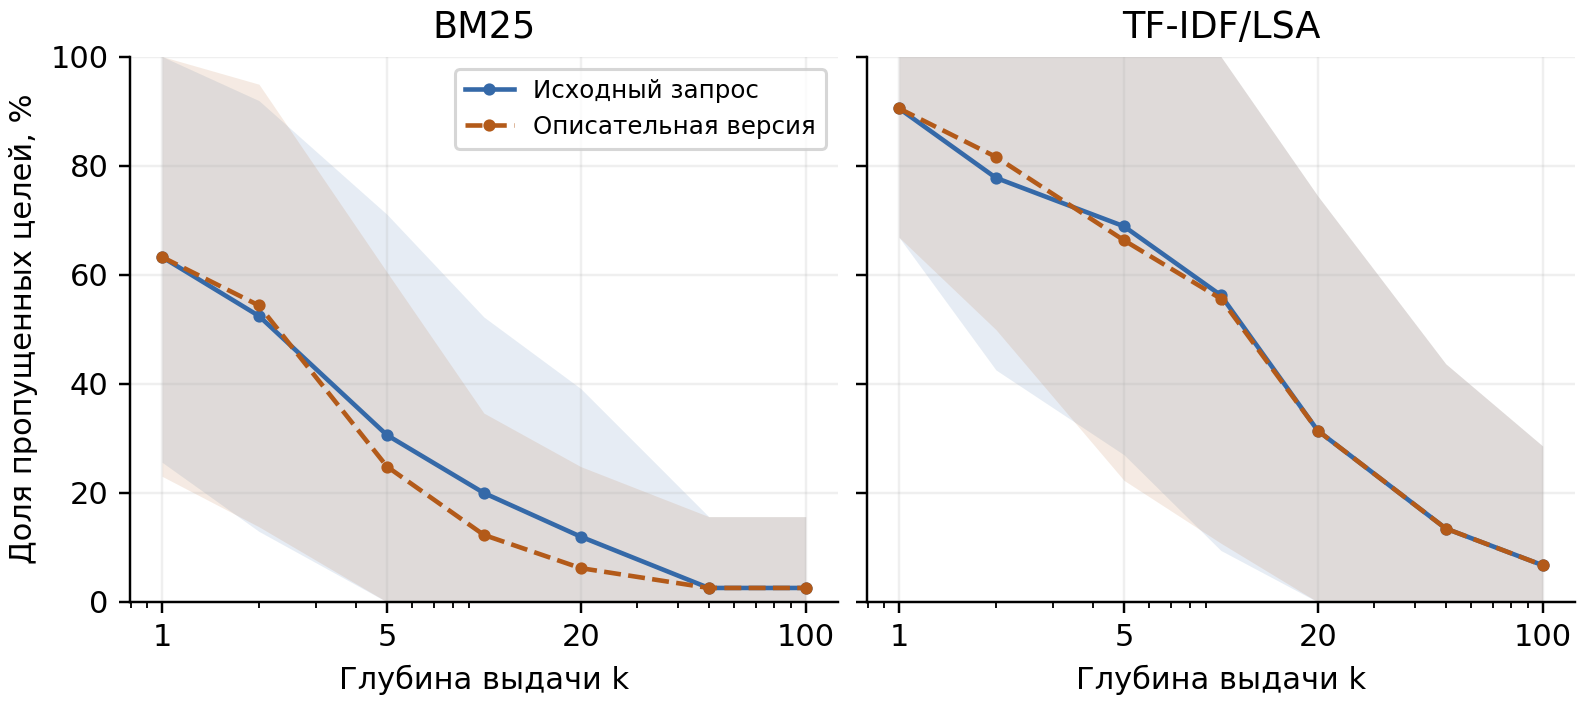
\includegraphics[width=\linewidth]{figures/search-target-coverage.png}
\caption{Доля пропущенных кандидатных целей $1-C_k$ при разной глубине выдачи. Линии показывают среднее по 26 вопросам, полосы --- одно выборочное стандартное отклонение с ограничением отображения диапазоном $[0,100]$. Полосы характеризуют разброс между вопросами.}
\label{fig:search-coverage}
\end{figure}

На рисунке~\ref{fig:search-coverage} меняется глубина выдачи при фиксированном ранжировании. Это диагностика покрытия по сохранённым позициям целей. Вопросы могут иметь общие статьи, поэтому показанный разброс не предполагает независимости наблюдений. Для последней серии, остановленной после полнотекстового судьи, прямой поиск ещё не выполнен.

\subsection{Зависимость ошибки поиска от размерности LSA}\label{sec:lsa-complexity}

Варьируем число компонент LSA при фиксированных корпусе, TF-IDF и исходных запросах. Используем все 33 исходных вопроса с завершённой проверкой и 86 кандидатными целевыми парами. Отбор по сохранению целей после переформулирования здесь не применяется, поэтому эта выборка отличается от 26 парных вопросов раздела~\ref{sec:retrieval}.

Рассмотрены размерности 32, 64, 128 и 256 при \texttt{random\_state=42}. Для 128 компонент используются исходные преобразование и векторы документов; все сохранённые позиции целей воспроизвелись точно. Для остальных размерностей заново вычислена SVD на той же TF-IDF-матрице. Размер выдачи фиксирован, $k=20$. Ошибка вопроса равна $1-C_{20}$.

\begin{table}[t]
\centering
\caption{Ошибка поиска при разной размерности LSA на 33 исходных вопросах. Приведены число найденных пар из 86, средняя доля пропусков и выборочное стандартное отклонение по вопросам.}
\label{tab:lsa-complexity}
\begin{tabular}{rrr}
\toprule
Компоненты & Найденные пары & Доля пропусков, \% \\
\midrule
32 & 36/86 & $56.9\pm45.2$ \\
64 & 47/86 & $41.9\pm44.4$ \\
128 & 51/86 & $33.9\pm42.7$ \\
256 & 58/86 & $26.1\pm38.6$ \\
\bottomrule
\end{tabular}
\end{table}

\begin{figure}[t]
\centering
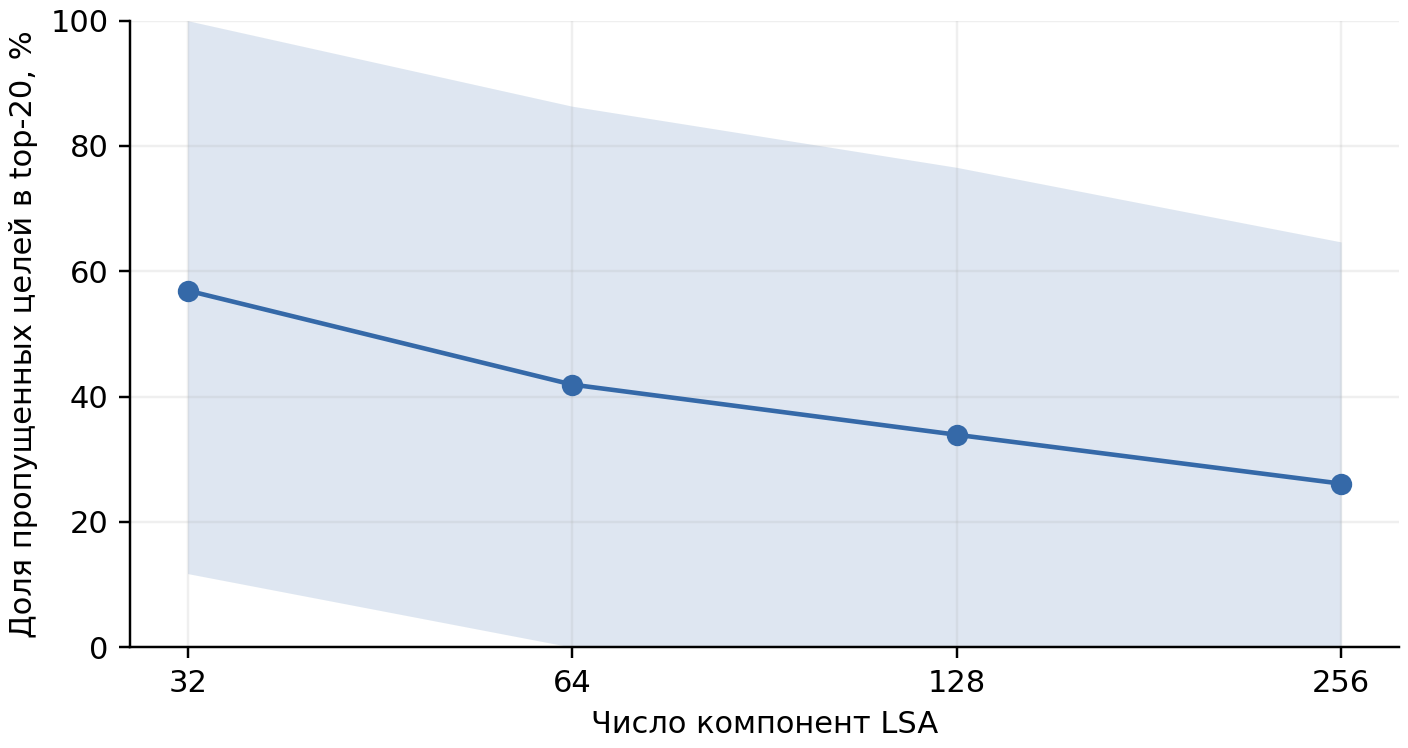
\includegraphics[width=0.9\linewidth]{figures/lsa-complexity.png}
\caption{Ошибка поиска от числа компонент LSA при фиксированном $k=20$. Линия показывает среднее по 33 вопросам, полоса --- одно выборочное стандартное отклонение, обрезанное границами $[0,100]$. Для каждой размерности использован один набор векторов; полоса описывает различия вопросов.}
\label{fig:lsa-complexity}
\end{figure}

На проверенной сетке увеличение размерности снижает среднюю долю пропусков с 56.9\% до 26.1\%. Большой межвопросный разброс сохраняется. Этот результат показывает зависимость наблюдаемой трудности задач от конфигурации прямого поиска. Вопросы и целевые пулы формировались с использованием исходного 128-компонентного индекса; окончательный выбор размерности и оценка переноса требуют отдельной контрольной выборки.

\subsection{Предварительный анализ лексического пересечения}

Цель эксперимента --- оценить, насколько совпадает лексика научных поисковых запросов и целевых статей в существующих бенчмарках. Такой анализ нужен для предварительной оценки того, насколько поисковый агент может находить целевые статьи, используя ключевые слова исходного запроса.

\paragraph{Данные и метод.}
Использованы ScholarQuest, AutoResearchBench и PaperPilot~\cite{pan2026scholarquest,xiong2026autoresearchbench,li2026paperpilot}. После исключения 30 вопросов настройки основная выборка содержит 2\,071 вопрос и 64\,865 пар «запрос --- целевая статья».

Из запроса автоматически выделяются содержательные выражения, удаляются служебные слова и нормализуются словоформы. Покрытие определяется как доля различных слов запроса, встретившихся в статье. Для вопросов с несколькими целями показатель рассчитывается отдельно для каждой статьи, затем усредняется внутри вопроса. Итоговые значения усредняются по вопросам; недоступные тексты исключаются из расчёта.

\paragraph{Заголовки и аннотации.}
Оценка получена для 64\,580 пар --- 99,6\% основной выборки.

\begin{table}[htbp]
\centering
\caption{Лексическое покрытие запроса в заголовке и аннотации целевой статьи.}
\label{tab:lexical-ta}
\small
\begin{tabular}{lrr}
\toprule
Бенчмарк & Оценено пар / всего & Покрытие слов \\
\midrule
ScholarQuest & 59\,851 / 59\,851 & 46,3\% \\
AutoResearchBench Deep & 535 / 535 & 10,8\% \\
AutoResearchBench Wide & 4\,121 / 4\,122 & 30,2\% \\
PaperPilot & 73 / 357 & 38,9\% \\
\bottomrule
\end{tabular}
\end{table}

Наименьшее покрытие наблюдается в AutoResearchBench Deep, вопросы которого строятся по косвенным деталям целевой статьи. Результат PaperPilot относится к ограниченной доступной части релиза.

\begin{figure}[htbp]
\centering
\IfFileExists{figures/lexical-gap-title_abstract.png}{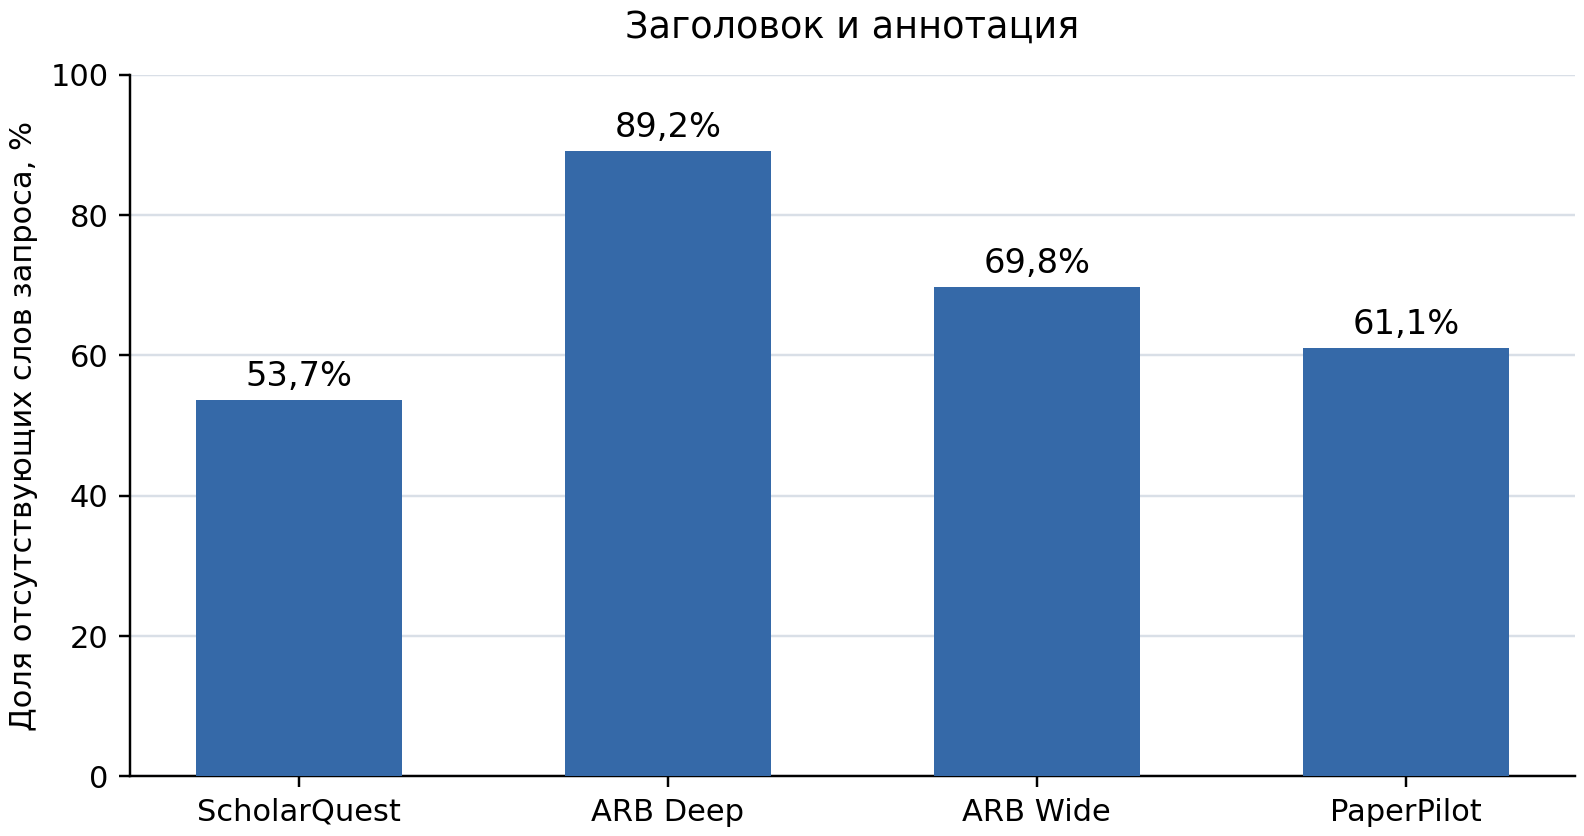
\includegraphics[width=0.9\linewidth]{figures/lexical-gap-title_abstract.png}}{%
% BEGIN INLINE FIGURE title_abstract
\begingroup\setlength{\unitlength}{0.8mm}
\begin{picture}(145,82)
\put(17,14){\line(1,0){124}}
\put(17,14){\line(0,1){60}}
\put(7,14){\makebox(8,0)[r]{\scriptsize 0}}
\put(17,14){\line(1,0){1}}
\put(7,26){\makebox(8,0)[r]{\scriptsize 20}}
\put(17,26){\line(1,0){1}}
\put(7,38){\makebox(8,0)[r]{\scriptsize 40}}
\put(17,38){\line(1,0){1}}
\put(7,50){\makebox(8,0)[r]{\scriptsize 60}}
\put(17,50){\line(1,0){1}}
\put(7,62){\makebox(8,0)[r]{\scriptsize 80}}
\put(17,62){\line(1,0){1}}
\put(7,74){\makebox(8,0)[r]{\scriptsize 100}}
\put(17,74){\line(1,0){1}}
\put(23,14){{\color[rgb]{0.21,0.41,0.66}\rule{14\unitlength}{32.22\unitlength}}}
\put(30,48.22){\makebox(0,0){\scriptsize 53,7\%}}
\put(30,8){\makebox(0,0){\scriptsize ScholarQuest}}
\put(54,14){{\color[rgb]{0.21,0.41,0.66}\rule{14\unitlength}{53.52\unitlength}}}
\put(61,69.52){\makebox(0,0){\scriptsize 89,2\%}}
\put(61,8){\makebox(0,0){\scriptsize ARB Deep}}
\put(85,14){{\color[rgb]{0.21,0.41,0.66}\rule{14\unitlength}{41.88\unitlength}}}
\put(92,57.88){\makebox(0,0){\scriptsize 69,8\%}}
\put(92,8){\makebox(0,0){\scriptsize ARB Wide}}
\put(116,14){{\color[rgb]{0.21,0.41,0.66}\rule{14\unitlength}{36.66\unitlength}}}
\put(123,52.66){\makebox(0,0){\scriptsize 61,1\%}}
\put(123,8){\makebox(0,0){\scriptsize PaperPilot}}
\put(17,80){\makebox(0,0)[l]{\scriptsize Доля отсутствующих слов запроса, \%}}
\end{picture}\endgroup
% END INLINE FIGURE title_abstract
}
\caption{Доля слов запроса, отсутствующих в заголовке и аннотации целевой статьи. ARB обозначает AutoResearchBench. Показатель равен единице минус покрытие и не является ошибкой поисковой системы.}
\label{fig:lexical-ta}
\end{figure}

\paragraph{Основной текст без библиографии и Related Work.}
Оценка выполнена на зафиксированном срезе из 12\,759 пар.

\begin{table}[htbp]
\centering
\caption{Лексическое покрытие запроса в основном тексте без библиографии и Related Work.}
\label{tab:lexical-body}
\small
\begin{tabular}{lrr}
\toprule
Бенчмарк & Оценено пар / всего & Покрытие слов \\
\midrule
ScholarQuest & 11\,766 / 59\,851 & 76,0\% \\
AutoResearchBench Deep & 93 / 535 & 54,7\% \\
AutoResearchBench Wide & 853 / 4\,122 & 72,2\% \\
PaperPilot & 47 / 357 & 81,5\% \\
\bottomrule
\end{tabular}
\end{table}

Полнотекстовый срез не сбалансирован по бенчмаркам и зависит от доступности статей. Поэтому приведённые значения характеризуют обработанные подмножества.

\begin{figure}[htbp]
\centering
\IfFileExists{figures/lexical-gap-body_clean.png}{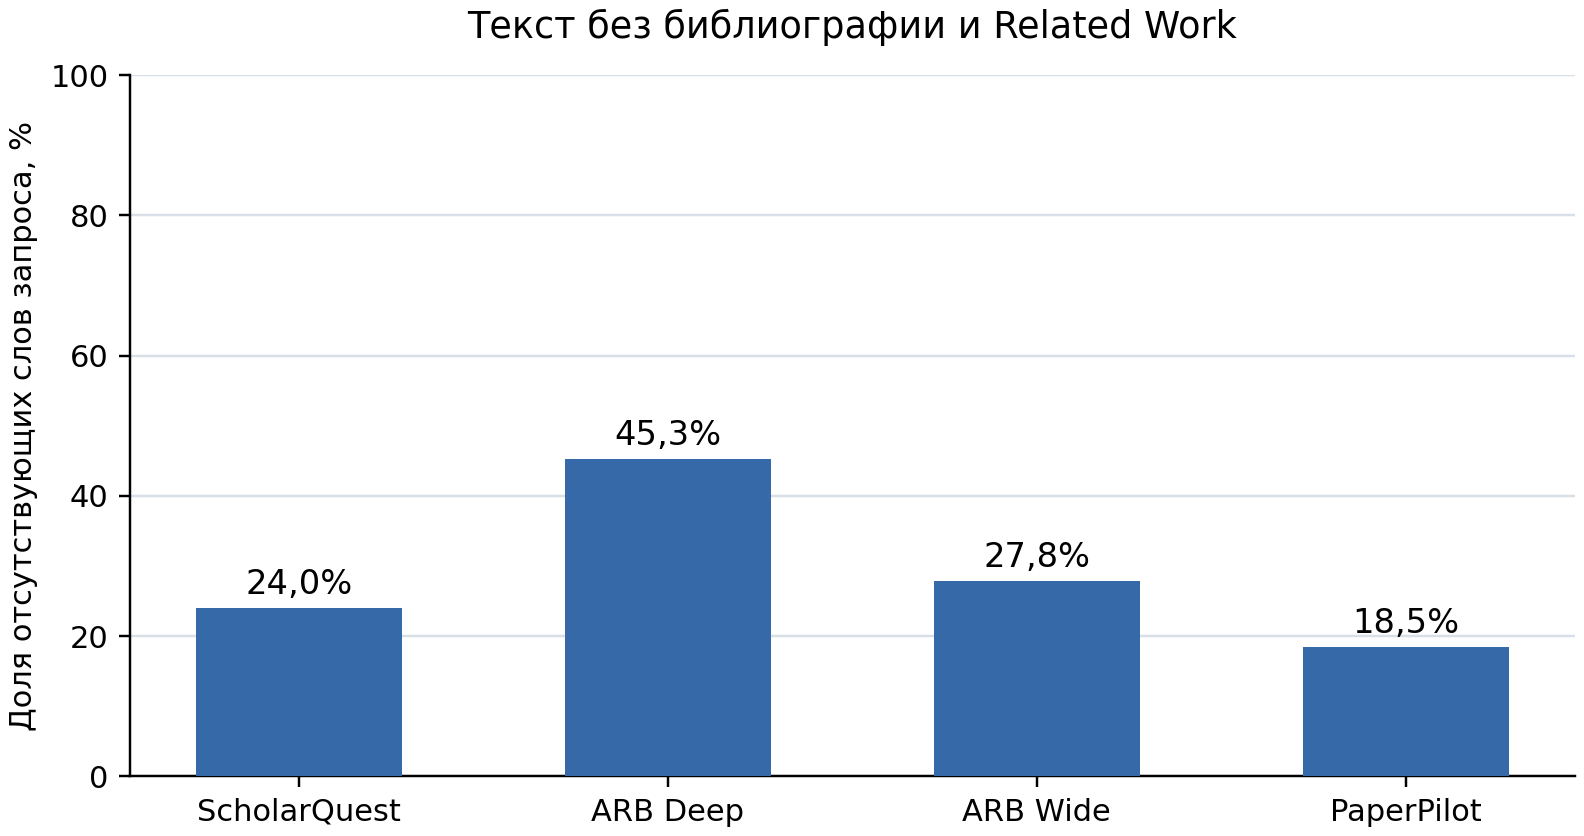
\includegraphics[width=0.9\linewidth]{figures/lexical-gap-body_clean.png}}{%
% BEGIN INLINE FIGURE body_clean
\begingroup\setlength{\unitlength}{0.8mm}
\begin{picture}(145,82)
\put(17,14){\line(1,0){124}}
\put(17,14){\line(0,1){60}}
\put(7,14){\makebox(8,0)[r]{\scriptsize 0}}
\put(17,14){\line(1,0){1}}
\put(7,26){\makebox(8,0)[r]{\scriptsize 20}}
\put(17,26){\line(1,0){1}}
\put(7,38){\makebox(8,0)[r]{\scriptsize 40}}
\put(17,38){\line(1,0){1}}
\put(7,50){\makebox(8,0)[r]{\scriptsize 60}}
\put(17,50){\line(1,0){1}}
\put(7,62){\makebox(8,0)[r]{\scriptsize 80}}
\put(17,62){\line(1,0){1}}
\put(7,74){\makebox(8,0)[r]{\scriptsize 100}}
\put(17,74){\line(1,0){1}}
\put(23,14){{\color[rgb]{0.21,0.41,0.66}\rule{14\unitlength}{14.40\unitlength}}}
\put(30,30.4){\makebox(0,0){\scriptsize 24,0\%}}
\put(30,8){\makebox(0,0){\scriptsize ScholarQuest}}
\put(54,14){{\color[rgb]{0.21,0.41,0.66}\rule{14\unitlength}{27.18\unitlength}}}
\put(61,43.18){\makebox(0,0){\scriptsize 45,3\%}}
\put(61,8){\makebox(0,0){\scriptsize ARB Deep}}
\put(85,14){{\color[rgb]{0.21,0.41,0.66}\rule{14\unitlength}{16.68\unitlength}}}
\put(92,32.68){\makebox(0,0){\scriptsize 27,8\%}}
\put(92,8){\makebox(0,0){\scriptsize ARB Wide}}
\put(116,14){{\color[rgb]{0.21,0.41,0.66}\rule{14\unitlength}{11.10\unitlength}}}
\put(123,27.1){\makebox(0,0){\scriptsize 18,5\%}}
\put(123,8){\makebox(0,0){\scriptsize PaperPilot}}
\put(17,80){\makebox(0,0)[l]{\scriptsize Доля отсутствующих слов запроса, \%}}
\end{picture}\endgroup
% END INLINE FIGURE body_clean
}
\caption{Доля слов запроса, отсутствующих в основном тексте без библиографии и Related Work. ARB обозначает AutoResearchBench. Оценка относится к доступному срезу каждого бенчмарка.}
\label{fig:lexical-body}
\end{figure}

\paragraph{Ограничения.}
Покрытие измеряет совпадение слов, а не смысловую эквивалентность терминов или выполнение требований запроса. Автоматическое выделение выражений может включать общие слова и объединять отдельные понятия. Для вопросов с несколькими целями среднее скрывает различия между статьями. Связь полученного показателя с успешностью поисковых систем в этом эксперименте не проверялась.

\section{Discussion}\label{sec:disc}

Фабрика получила вопросы с одним и несколькими кандидатными ответами и сохраняет происхождение каждой записи. Повторение шести формулировок при разных затравках показывает необходимость дедупликации перед выпуском набора. Число записей до этой процедуры завышает разнообразие запросов.

Проверка описательных версий выявила два разных ограничения. Часть запросов теряет прежние цели или допускает дополнительные ответы. При сохранении целей прямой поиск может по-прежнему находить их на высоких позициях. Поэтому сохранение релевантности и увеличение поисковой сложности следует оценивать раздельно.

Разметка получена моделью-судьёй на ограниченных пулах. Включение верхней выдачи в проверку помогает обнаруживать альтернативные ответы, но связывает наблюдаемый состав целей с выбранными методами поиска. Цели за пределами проверенного пула остаются неизвестными. Показатель $C_k$ измеряет покрытие этого пула; полнота поиска по всему корпусу не установлена.

Увеличение размерности LSA заметно улучшило покрытие известных целей. Поэтому поисковая сложность должна оцениваться относительно явно заданных конфигураций базовых методов.

Серии использовались для разработки фабрики и формулировок запросов. Переформулирование получает обратную связь от BM25 на этих же вопросах, поэтому оценка переноса на новые задачи требует отложенной выборки. Окончательная граница сложности и независимая контрольная выборка ещё не зафиксированы. Для оценки качества выпущенного набора нужны единый протокол принятия, независимая проверка разметки и сравнение с агентными системами на зафиксированных задачах. Текущие эксперименты устанавливают свойства генерации и её ошибки, а преимущество графового решателя остаётся открытым вопросом.

\section{Conclusion}\label{sec:concl}

Разработана фабрика поисковых задач по группам статей в графе цитирований. Получены 45 различных текстов вопросов с сохранёнными кандидатными ответами и результатами полнотекстовых проверок. Анализ показал, что описательное переформулирование требует повторной проверки ответов и в проведённой серии не обеспечило ожидаемого усложнения прямого поиска. Дальнейшая работа включает смысловую дедупликацию, независимую проверку разметки и сравнение поисковых агентов на зафиксированном наборе задач.

\bibliographystyle{unsrtnat}
\bibliography{references}

%%%%%%%%%%%%%%%%%%%%%%%%%%%%%%%%%%%%%%%%%%%%%%%%%%%%%%%%%%%%

\end{document}
